% !TeX root = ../analisi_2.tex

\section{Estremi liberi e formula di Taylor}

\subsection{Estremi relativi e condizione necessaria del 1° ordine}

\begin{definition}
Sia $f : A \subseteq \mathbb{R}^2 \to \mathbb{R}$, $A \neq \emptyset$ aperto.

$(x_0, y_0) \in A$ si dice \underline{pto di minimo relativo} per $f$ se $\exists I_\delta(x_0, y_0)$ tale che:
\[
f(x, y) \ge f(x_0, y_0) \quad \forall (x, y) \in I_\delta(x_0, y_0)
\]
\[
\Downarrow
\]
\[
f(x, y) - f(x_0, y_0) \ge 0
\]
\end{definition}

\begin{theorem}[Cond. nec. del 1° ordine]
Sia $f : A \subseteq \mathbb{R}^2 \to \mathbb{R}$, $A$ aperto, $A \neq \emptyset$, $(x_0, y_0) \in A$ estremo relativo.

Allora se $f$ è derivabile nel punto $\implies \nabla f(x_0, y_0) = (0, 0)$ \pencilnote{ovvero gli estremi relativi hanno $\text{grad} = 0$}, cioè
\[
\begin{cases}
f_x(x_0, y_0) = 0 \\
f_y(x_0, y_0) = 0
\end{cases} \qquad \text{\pencilnote{chiameremo punti critici le sol. del sist.}}
\]
\end{theorem}

\begin{proof}
\begin{center}
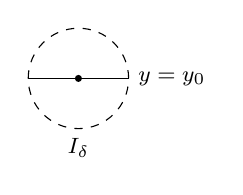
\begin{tikzpicture}[scale=0.85]
    \draw[dashed] (0,0) circle (0.75);
    \draw (-0.75,0) -- (0.75,0) node[right] {\footnotesize $y = y_0$};
    \fill (0,0) circle (1.5pt);
    \node[below] at (0,-0.75) {\footnotesize $I_\delta$};
\end{tikzpicture}
\end{center}
$\Delta f$ ha segno \pencilnote{(suppongo $\ge 0$)}.

Se considero in $y = y_0$, $f(x, y_0)$ per Fermat su questo segmento il punto ha derivata $= 0$ \pencilnote{(la der. in quel punto)}.
\end{proof}

\begin{proof}[Dimostrazione per def. (stesso teo)]
$\exists I_\delta(x_0, y_0) : \Delta f \ge 0$ in $I_\delta(x_0, y_0)$ \pencilnote{(se assumo che è minimo)}
\[
\implies g(x) = f(x, y_0), \qquad x \in ]x_0 - \delta, x_0 + \delta[
\]
ha estremo relativo in $x = x_0$.

\pencilnote{Se fisso una variabile, facendo la der. faccio la parziale, quindi il gradiente mi dice che la derivata su quel diametro è $= 0$ (per Fermat è minimo).}
\end{proof}

\subsection{Esercizi sugli estremi e Matrice Hessiana}

\begin{esercizio}[EXE 1]
\[
f(x, y) = e^{-x^2 + 2x - y^2} \qquad C = \{ x^2 + y^2 \le 4, \ 0 \le x \le y \}
\]
\end{esercizio}

\begin{esercizio}[EXE 2]
\[
f(x, y) = (x^2 - y^2)(1 - x^2)
\]
$T =$ triangolo di vertici $(-1, 1)$, $(1, 1)$, $(-1, -1)$.
\end{esercizio}

\subsubsection*{Recap}

\begin{definition}
Sia $f : A \subseteq \mathbb{R}^2 \to \mathbb{R}$, $A \neq \emptyset$, $A$ aperto. $(x_0, y_0) \in A$.

Si dice \underline{pto di est. relativo} se:
\[
\exists I_\delta(x_0, y_0) : \Delta f(x_0, y_0)
\begin{cases}
\ge 0 \to \text{min rel} \\
\le 0 \to \text{max rel}
\end{cases}
\quad \text{in } I_\delta(x_0, y_0)
\]
ovvero $(f(x, y) - f(x_0, y_0))$ ha segno.
\end{definition}

\begin{theorem}[Teo cond. nec. del 1° ordine]
Sia $f : A \subseteq \mathbb{R}^2 \to \mathbb{R}$, $A \neq \emptyset$, $A$ aperto e se $(x_0, y_0) \in A$ è un estremo relativo. Allora se $\exists \nabla f(x_0, y_0) \implies$
\[
\begin{cases}
f_x(x_0, y_0) = 0 \\
f_y(x_0, y_0) = 0
\end{cases}
\]
\end{theorem}

\begin{example*}[Controesempio]
\[
f(x, y) = x^2 - y^2
\]
Troviamo i pti critici:
\[
\nabla f(x, y) = 0 \iff \begin{cases} f_x = 0 \\ f_y = 0 \end{cases} \iff \begin{cases} 2x = 0 \\ -2y = 0 \end{cases} \to (0, 0)
\]
È un estremo rel.?
\[
\Delta f(0, 0) = \underbrace{x^2 - y^2}_{f} - \underbrace{0}_{f(0, 0)} = x^2 - y^2 \ge 0 \implies y^2 \le x^2 \implies |y| \le |x|
\]
\begin{center}
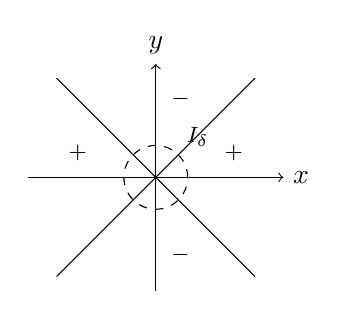
\begin{tikzpicture}[scale=0.9]
    \draw[->] (-1.8,0) -- (1.8,0) node[right] {$x$};
    \draw[->] (0,-1.6) -- (0,1.6) node[above] {$y$};
    \draw (-1.4,-1.4) -- (1.4,1.4);
    \draw (-1.4,1.4) -- (1.4,-1.4);
    \draw[dashed] (0,0) circle (0.45);
    \node[above right] at (0.3,0.3) {\footnotesize $I_\delta$};
    \node at (1.1,0.35) {\footnotesize $+$};
    \node at (-1.1,0.35) {\footnotesize $+$};
    \node at (0.35,1.1) {\footnotesize $-$};
    \node at (0.35,-1.1) {\footnotesize $-$};
\end{tikzpicture}
\end{center}
In un qualunque $I_\delta(0, 0)$ non ho segno $\implies (0, 0)$ non è né un max né un min rel.

\pencilnote{(Blocco 1 comp.: per $f(x, 0) \to f(x) = x^2 \implies (0, 0)$ è minimo rel.; per $f(0, y) \to f(y) = -y^2 \implies (0, 0)$ è max rel. Assurdo.)}
\end{example*}

\begin{esercizio}[EXE in $\mathbb{R}$]
$f(x) : [a, b] \to \mathbb{R}$ deriv. in $[a, b]$:
\[
f(x) = e^{x^2} - 3x^2 \quad \text{in } [0, 1]
\]
Candidati \pencilnote{(ad estr. rel.)}:
\begin{enumerate}
    \item $x = 0, \ x = 1$ \quad ``Tappi''
    \item $f'(x) = 0$
    \item pti di non der.
\end{enumerate}
\[
f'(x) = 2x e^{x^2} - 6x = 0 \implies e^{x^2} = 3 \implies x^2 = \log 3
\]
\[
x = 0, \ x = 1 \to f(0) = 0, \quad f(1) = e - 3
\]
\[
x = \pm\sqrt{\log 3} \to x = +\sqrt{\log 3}
\]
\end{esercizio}

\begin{esercizio}[EXE in $\mathbb{R}^2$ (EXE 1)]

\noindent\begin{minipage}{\linewidth}
\centering
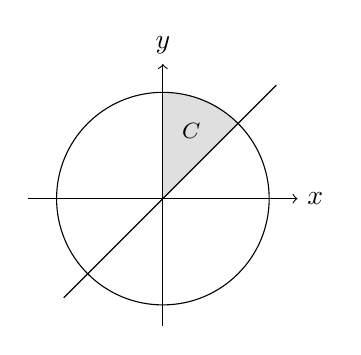
\begin{tikzpicture}[scale=0.9]
    \fill[gray!25] (0,0) -- (0,1.5) arc (90:45:1.5) -- cycle;
    \draw[->] (-1.9,0) -- (1.9,0) node[right] {$x$};
    \draw[->] (0,-1.8) -- (0,1.9) node[above] {$y$};
    \draw (0,0) circle (1.5);
    \draw (-1.4,-1.4) -- (1.6,1.6);
    \node at (0.4,0.95) {\footnotesize $C$};
\end{tikzpicture}
\end{minipage}

\vspace{0.5em}
\noindent$\implies C$ è un compatto $\to f(x, y) = e^{-x^2 + 2x - y^2}$ è continua per il teo del diff. totale.


\[
\begin{cases}
f_x = 0 \\
f_y = 0
\end{cases}
\iff
\begin{cases}
(-2x + 2) e^{-x^2 + 2x - y^2} = 0 \\
(-2y) e^{-x^2 + 2x - y^2} = 0
\end{cases}
\implies
\begin{cases}
x = 1 \\
y = 0
\end{cases}
\implies P(1, 0) \notin C
\]
\pencilnote{In $\mathbb{R}^2$ i ``tappi'' $\to$ curve (frontiera).}

\textbf{Su $C_1$} (intero disco di raggio $2$): $\partial C_1 = \gamma$, $\gamma(t) = (2\cos t, 2\sin t)$, $t \in [0, 2\pi]$:
\[
f(\gamma(t)) = e^{-4 + 4\cos t} = g(t) \qquad t \in [0, 2\pi]
\]
$Q_1 = (x(0), y(0)) = (2, 0)$ \quad $|$ \quad $P(1, 0)$
\begin{itemize}
    \item $g'(t) = 0 \qquad t \in ]0, 2\pi[$
    \[
    g'(t) = e^{-4 + 4\cos t} \cdot (-4\sin t) = 0 \qquad t \in ]0, 2\pi[ \implies \sin t = 0 \implies t = \pi
    \]
    $Q_2 = (x(\pi), y(\pi)) = (-2, 0)$
\end{itemize}
\begin{align*}
f(P) &= f(1, 0) = e \to \text{max ass.} \\
f(Q_1) &= f(2, 0) = 1 \\
f(Q_2) &= f(-2, 0) = 1/e^8 \to \text{min ass.}
\end{align*}

\textbf{In $C$:}
\begin{center}
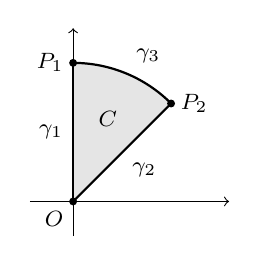
\begin{tikzpicture}[scale=1.1]
    \fill[gray!20] (0,0) -- (0,1.6) arc (90:45:1.6) -- cycle;
    \draw[->] (-0.5,0) -- (1.8,0);
    \draw[->] (0,-0.4) -- (0,2.0);
    \draw[thick] (0,0) -- node[left] {\footnotesize $\gamma_1$} (0,1.6);
    \draw[thick] (0,0) -- node[below right] {\footnotesize $\gamma_2$} (1.131,1.131);
    \draw[thick] (0,1.6) arc (90:45:1.6) node[midway, above right] {\footnotesize $\gamma_3$};
    \fill (0,0) circle (1.3pt) node[below left] {\footnotesize $O$};
    \fill (0,1.6) circle (1.3pt) node[left] {\footnotesize $P_1$};
    \fill (1.131,1.131) circle (1.3pt) node[right] {\footnotesize $P_2$};
    \node at (0.4,0.95) {\footnotesize $C$};
\end{tikzpicture}
\end{center}
Lista:
\[
O = (0, 0), \qquad P_1 = (0, 2), \qquad P_2 = \left( 2\cos\frac{\pi}{4}, 2\sin\frac{\pi}{4} \right) = (\sqrt{2}, \sqrt{2})
\]
Lo studio su $\gamma_3$ è già stato fatto prima (su $C_1$).
\[
\gamma_1 = \begin{cases} x = 0 \\ y = t \end{cases} \quad t \in [0, 2], \qquad
\gamma_2 = \begin{cases} x = t \\ y = t \end{cases} \quad t \in [0, \sqrt{2}]
\]
\begin{itemize}
    \item $f(\gamma_1(t)) = e^{-t^2}$ in $]0, 2[$ non ha pti critici interni \pencilnote{(potrei considerare $t = 0$ e $t = 2$ ma già li ho considerati)}.
    \item $f(\gamma_2(t)) = e^{-2t^2 + 2t} = g(t) \qquad t \in ]0, \sqrt{2}[$
    \[
    g'(t) = e^{-2t^2 + 2t} (-4t + 2) = 0 \implies t = \frac{2}{4} = \frac{1}{2} \in ]0, \sqrt{2}[ \implies P_3 = \left( \frac{1}{2}, \frac{1}{2} \right)
    \]
\end{itemize}
Lista: $O, P_1, P_2, P_3$:
\[
f(O) = 1, \qquad
f(P_1) = 1/e^4 \ \text{(min ass.)}, \qquad
f(P_2) = e^{-4 + 2\sqrt{2}} = \frac{1}{e^{4 - 2\sqrt{2}}}, \qquad
f(P_3) = e^{1/2} \ \text{(max ass.)}
\]
\end{esercizio}

\subsubsection*{Cond. necessaria del II° ordine (Analisi 1)}

$f : [a, b] \to \mathbb{R}$, $f \in C^2([a, b])$, se $x_0$ è un estr. $\implies$
\[
\begin{cases}
f'(x_0) = 0 \\
f''(x_0) \begin{cases} \ge 0 & \text{min} \\ \le 0 & \text{max} \end{cases}
\end{cases}
\]

\begin{definition}[Matrice Hessiana]
Sia $f : A \subseteq \mathbb{R}^2 \to \mathbb{R}$, $A \neq \emptyset$ e $A$ aperto, derivabile. Allora sono definite due funzioni:
\[
\begin{cases}
f_x : A \to \mathbb{R} \\
f_y : A \to \mathbb{R}
\end{cases}
\qquad \text{poiché } \exists \nabla f(x, y) \ \forall (x, y) \in A
\]
Se $f_x$ e $f_y$ sono a loro volta derivabili in $A$, risulta:
\begin{itemize}
    \item $f_x \xrightarrow{\frac{\partial}{\partial x}} f_{xx}(x, y)$ \quad (pura), \qquad $f_x \xrightarrow{\frac{\partial}{\partial y}} f_{xy}(x, y)$ \quad (mista)
    \item $f_y \xrightarrow{\frac{\partial}{\partial x}} f_{yx}(x, y)$ \quad (mista), \qquad $f_y \xrightarrow{\frac{\partial}{\partial y}} f_{yy}(x, y)$ \quad (pura)
\end{itemize}
\[
\implies D^2 f = \begin{pmatrix} \nabla f_x(x, y) \\ \nabla f_y(x, y) \end{pmatrix} = \begin{pmatrix} f_{xx}(x, y) & f_{xy}(x, y) \\ f_{yx}(x, y) & f_{yy}(x, y) \end{pmatrix}
\]
che si chiama \underline{Matrice Hessiana}.
\[
H_f(x, y) = \det D^2 f(x, y) = f_{xx} f_{yy} - f_{xy} f_{yx}
\]
si chiama \underline{Determinante Hessiano} o \underline{Hessiano}.

Sulla diagonale magg.: derivate \underline{pure}; nel rest. della matrice: le \underline{miste}.
\end{definition}

\begin{esercizio}
$f(x, y) = x^4 y - e^{xy}$, \quad $D^2 f(1, 0) = ?$
\begin{align*}
f_x &= 4x^3 y - y e^{xy} &\implies f_{xx} &= 12x^2 y - y^2 e^{xy}, \quad f_{xy} = 4x^3 - x y e^{xy} - e^{xy} \\
f_y &= x^4 - x e^{xy} &\implies f_{yx} &= 4x^3 - x y e^{xy} - e^{xy}, \quad f_{yy} = -x^2 e^{xy}
\end{align*}
Valutate in $(1, 0)$:
\[
f_{xx} = 0, \quad f_{xy} = 3, \quad f_{yx} = 3, \quad f_{yy} = -1
\]
\[
D^2 f(1, 0) = \begin{pmatrix} 0 & 3 \\ 3 & -1 \end{pmatrix} \implies H_f(1, 0) = -9
\]
\end{esercizio}

\begin{oss}
In questo caso le miste sono uguali, dunque la matrice $D^2 f(x, y)$ è simmetrica $\implies$ è diagonalizzabile.
\end{oss}

\subsection{Teorema di Schwarz e operatori differenziali}

\begin{theorem}[Teo di Schwarz (s.d.)]
Sia $f : A \subseteq \mathbb{R}^2 \to \mathbb{R}$, $A \neq \emptyset$, $A$ aperto. Sia $f$ derivabile 2 volte in $A$, sia $(x_0, y_0) \in A$ t.c. $f_{xy}$ e $f_{yx}$ sono continue in $(x_0, y_0)$.

Allora
\[
f_{xy}(x_0, y_0) = f_{yx}(x_0, y_0)
\]
Ovvero $f \in C^2 \implies D^2 f$ simmetrica! \quad ($\not\impliedby$)
\end{theorem}

\begin{oss}
\underline{Non} è vero che se le miste coincidono allora $f_{xy}$ e $f_{yx}$ sono continue.
\end{oss}

\begin{example*}[Controesempio]
\[
f(x, y) = \begin{cases}
\dfrac{x^3 y - x y^3}{x^2 + y^2} & \text{se } (x, y) \neq (0, 0) \\
0 & \text{se } (x, y) = (0, 0)
\end{cases}
\]
Provare che:
\begin{itemize}
    \item $f$ è derivabile 2 volte in $(0, 0)$ e che $f_{xy}(0, 0) \neq f_{yx}(0, 0)$ e $f_{xy}$ e $f_{yx}$ non sono continue.
\end{itemize}
\end{example*}

\subsubsection*{Conseguenze}

Sia $F : A \subseteq \mathbb{R}^n \to \mathbb{R}^n$, $A \neq \emptyset$, aperto \pencilnote{(campo vettoriale, funzione da $\mathbb{R}^n \to \mathbb{R}^n$)}:
\[
\underbrace{F(x_1, x_2, \dots, x_n)}_{x \in A} = \underbrace{(F_1(x), F_2(x), \dots, F_n(x))}_{n \text{ funz. di } n \text{ variabili}} \in \mathbb{R}^n
\]
in $\mathbb{R}^3$: $F(x, y, z) = (F_1(x, y, z), F_2(x, y, z), F_3(x, y, z))$.

\begin{itemize}
    \item La \underline{divergenza} è per definizione:
    \[
    \underbrace{\operatorname{div} F(x, y, z)}_{\text{è uno scalare}} = \frac{\partial F_1}{\partial x}(x, y, z) + \frac{\partial F_2}{\partial y}(x, y, z) + \frac{\partial F_3}{\partial z}(x, y, z) \qquad (\nabla \cdot F)
    \]
    \pencilnote{(confezionata nell'Hp che $F_i$ siano derivabili)}

    Nel caso di $n$ variabili:
    \[
    \operatorname{div} F = \sum_{k=1}^n \frac{\partial F_k}{\partial x_k} = \frac{\partial F_1}{\partial x_1} + \frac{\partial F_2}{\partial x_2} + \dots + \frac{\partial F_n}{\partial x_n}
    \]

    \item Il \underline{rotore} è per def.:
    \[
    \underbrace{\operatorname{rot} F}_{\text{è un vettore}} = \begin{vmatrix}
    \mathbf{i} & \mathbf{j} & \mathbf{k} \\
    \dfrac{\partial}{\partial x} & \dfrac{\partial}{\partial y} & \dfrac{\partial}{\partial z} \\
    F_1 & F_2 & F_3
    \end{vmatrix} = \left( \frac{\partial F_3}{\partial y} - \frac{\partial F_2}{\partial z}, \ \frac{\partial F_1}{\partial z} - \frac{\partial F_3}{\partial x}, \ \frac{\partial F_2}{\partial x} - \frac{\partial F_1}{\partial y} \right)
    \]
\end{itemize}

\begin{prop*}[Conseguenza di Schwarz]
Come conseguenza di Schwarz, otteniamo: sia $f \in C^2(A)$, $A \subseteq \mathbb{R}^3$, aperto, $A \neq \emptyset$.
\begin{enumerate}
    \item $\operatorname{rot}(\nabla f) = 0 \quad (\text{I})$
    \item $\operatorname{div}(\operatorname{rot} F) = 0 \quad (\text{II}) \quad \text{\pencilnote{($F \in C^2$)}}$
\end{enumerate}
\end{prop*}

\begin{proof}
\begin{align*}
\text{(I)}\quad \operatorname{rot}(\nabla f) &= \operatorname{rot}\left( \frac{\partial f}{\partial x}, \frac{\partial f}{\partial y}, \frac{\partial f}{\partial z} \right) = \operatorname{rot}(f_x, f_y, f_z) = (f_{zy} - f_{yz}, f_{xz} - f_{zx}, f_{yx} - f_{xy}) = (0, 0, 0) \\[6pt]
\text{(II)}\quad \operatorname{div}(\operatorname{rot} F) &= \operatorname{div}\left( \frac{\partial F_3}{\partial y} - \frac{\partial F_2}{\partial z}, \frac{\partial F_1}{\partial z} - \frac{\partial F_3}{\partial x}, \frac{\partial F_2}{\partial x} - \frac{\partial F_1}{\partial y} \right) = \\
&= \frac{\partial^2 F_3}{\partial x \partial y} - \frac{\partial^2 F_2}{\partial x \partial z} + \frac{\partial^2 F_1}{\partial y \partial z} - \frac{\partial^2 F_3}{\partial y \partial x} + \frac{\partial^2 F_2}{\partial z \partial x} - \frac{\partial^2 F_1}{\partial z \partial y} = 0
\end{align*}
\pencilnote{(poiché le comp. $F_x, F_y, F_z \in C^2$) per Schwarz.}
\end{proof}

\subsection{Formula di Taylor}

\begin{theorem}[Formula di Taylor con il resto di Lagrange]
Sia $f : A \subseteq \mathbb{R}^2 \to \mathbb{R}$, $A \neq \emptyset$, $A$ aperto e sia $f \in C^2(A)$.

Sia $P = (x, y) \in A$ e $(h, k) : (x + h, y + k) \in A$ e supponiamo che il segmento che congiunge $P$ e $P + (h, k)$ sia tutto contenuto in $A$.

Allora $\exists \theta \in [0, 1]$:
\[
\begin{aligned}
f(x + h, y + k) ={}& f(x, y) + f_x(x, y)\, h + f_y(x, y)\, k \\
&+ \frac{1}{2} \left[
f_{xx}(x + \theta h, y + \theta k)\, h^2 \right.\\
&\qquad \left. + 2 f_{xy}(x + \theta h, y + \theta k)\, hk \right.\\
&\qquad \left. + f_{yy}(x + \theta h, y + \theta k)\, k^2
\right]
\end{aligned}
\]
In not. vettoriale: $\underbrace{x}_{\text{vettore}} = (x, y)$, $v = (h, k)$
\[
f(x + v) = f(x) + \langle \nabla f(x), v \rangle + \frac{1}{2} \langle D^2 f(x + \theta v)\, v, v \rangle
\]
\end{theorem}

\begin{proof}
Sia $\gamma(t) = (x + th, y + tk)$, $t \in [0, 1]$, tale segmento $\implies \gamma'(t) = (h, k)$.

Consideriamo $F(t) = f(\gamma(t)) = f(x + th, y + tk)$.

\begin{center}
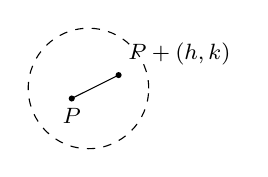
\begin{tikzpicture}[scale=0.85]
    \draw[dashed] (0,0) circle (0.9);
    \fill (-0.25,-0.15) circle (1.3pt) node[below] {\footnotesize $P$};
    \fill (0.45,0.2) circle (1.3pt) node[above right] {\footnotesize $P + (h,k)$};
    \draw (-0.25,-0.15) -- (0.45,0.2);
\end{tikzpicture}
\end{center}

\pencilnote{Poiché $f \in C^2 \to F$ è di classe $C^2([0, 1])$ per il teo del diff. totale (applicato 2 volte) $\implies$}

$\implies$ per il teo di deriv. delle funz. comp. risulta:
\begin{align*}
F'(t) &= f_x(\gamma(t))\, h + f_y(\gamma(t))\, k = f_x(x + th, y + tk)\, h + f_y(x + th, y + tk)\, k \\[4pt]
F''(t) &= f_{xx}(\gamma(t))\, h^2 + f_{xy}(\gamma(t))\, kh + f_{yx}(\gamma(t))\, hk + f_{yy}(\gamma(t))\, k^2 = \\
&= f_{xx}(\gamma(t))\, h^2 + 2 f_{xy}(\gamma(t))\, kh + f_{yy}(\gamma(t))\, k^2 \qquad t \in [0, 1]
\end{align*}
Usando la formula di Taylor con il resto di Lagrange in $t = 0$ per $F$, si ha $\exists \theta \in [0, 1]$:
\[
F(t) = F(0) + F'(0) \cdot t + \frac{F''(\theta)}{2} t^2 \qquad t \in [0, 1]
\]
per $t = 1$ si ha:
\[
F(1) = F(0) + F'(0) + \frac{F''(\theta)}{2}
\]
Sostituendo le loro espressioni si ottiene la formula di Taylor del 2° ordine con resto di Lagrange.
\end{proof}

\begin{theorem}[Form. di Taylor con il resto di Peano al II ordine]
Sia $f : A \subseteq \mathbb{R}^2 \to \mathbb{R}$, $A \neq \emptyset$, e aperto e sia $f \in C^2(A)$.

Sia $P = (x, y) \in A$ e siano $(h, k) : (x + h, y + k) \in A$ e t.c. il segmento che collega $P$ e $P + (h, k)$ è contenuto in $A$.

Allora vale la seg. formula di Taylor con il resto di Peano al II ordine:
\[
f(x + h, y + k) = f(x, y) + f_x(x, y)\, h + f_y(x, y)\, k + \frac{1}{2} \left[ f_{xx}(x, y)\, h^2 + 2 f_{xy}(x, y)\, hk + f_{yy}(x, y)\, k^2 \right] + o(h^2 + k^2)
\]
\end{theorem}

\begin{proof}
(Dalla formula del resto di Lagrange)
\[
\implies f(x + h, y + k) = f(x, y) + f_x(x, y)\, h + f_y(x, y)\, k + \frac{1}{2} \underbrace{[\dots]}_{\text{termine } 2^\circ \text{ ordine di Lagr.}}
\]
Ma io voglio dim. che:
\[
f(x + h, y + k) = f(x, y) + f_x(x, y)\, h + f_y(x, y)\, k + \frac{1}{2} \left[ \text{termine II ordine Peano} \right] + o(h^2 + k^2)
\]
La Th risulta dim. se
\[
\text{termine II° ordine di Lagrange} = \text{termine II° ordine di Peano} + o(h^2 + k^2)
\]
\[
\Updownarrow
\]
\[
\frac{(\text{term. II° ordine Lagrange}) - (\text{term. II° ordine Peano})}{h^2 + k^2} \to 0 \qquad (\text{per } (h, k) \to (0, 0))
\]
Quindi si ha:
\begin{align*}
&\left[ f_{xx}(x + \theta h, y + \theta k) - f_{xx}(x, y) \right] \frac{h^2}{h^2 + k^2} + 2 \left[ f_{xy}(x + \theta h, y + \theta k) - f_{xy}(x, y) \right] \frac{hk}{h^2 + k^2} + \\
&+ \left[ f_{yy}(x + \theta h, y + \theta k) - f_{yy}(x, y) \right] \frac{k^2}{h^2 + k^2}
\end{align*}
Ma $(h, k) \to (0, 0)$. Dunque, poiché $f \in C^2 \implies$ le derivate sono continue $\implies$ le $[\dots]$ vanno a $0$. Allora devo dim. che le ``fraz'' sono limitate:
\[
\frac{h^2}{h^2 + k^2} \le 1, \qquad \frac{k^2}{h^2 + k^2} \le 1 \qquad \text{e} \qquad -1 \le \frac{2hk}{h^2 + k^2} \le 1
\]
\pencilnote{Infatti: $(h + k)^2 = h^2 + k^2 + 2hk \ge 0 \implies 2hk \ge -(h^2 + k^2) \implies -1 \le \dfrac{2hk}{h^2 + k^2}$; analogamente $(h - k)^2 = h^2 + k^2 - 2hk \ge 0 \implies 2hk \le h^2 + k^2 \implies \dfrac{2hk}{h^2 + k^2} \le 1$.}
\end{proof}

\subsection{Condizioni del II ordine}

Grazie alla form. di Tay si possono dim. i seg.:

\begin{theorem}[Cond. nec. al II ordine]
\pencilnote{($m = 2$, non vale in $\mathbb{R}^n$)}

Sia $f : A \subseteq \mathbb{R}^2 \to \mathbb{R}$, $A \neq \emptyset$ e aperto e sia $f \in C^2(A)$.
\begin{itemize}
    \item Se $(x_0, y_0) \in A$ è un punto di minimo relativo $\implies$
    \[
    \begin{cases}
    \nabla f(x_0, y_0) = (0, 0) \\
    H_f(x_0, y_0) \ge 0 \\
    f_{xx}(x_0, y_0) \ge 0
    \end{cases}
    \]
    \item Se $(x_0, y_0) \in A$ è un pto di max rel $\implies$
    \[
    \begin{cases}
    \nabla f(x_0, y_0) = (0, 0) \\
    H_f(x_0, y_0) \ge 0 \\
    f_{xx}(x_0, y_0) \le 0
    \end{cases}
    \]
\end{itemize}
\end{theorem}

\begin{proof}[Dim. condizione necessaria (II ordine)]
\pencilnote{(In Analisi 1: $\underbrace{f(x) - f(x_0)}_{\Delta f \ge 0 \text{ in } I_\delta(x_0)} = f'(x_0)(x - x_0) + \dfrac{f''(x_0)}{2}(x - x_0)^2 + o(x - x_0)^2 \ge 0 \implies \dfrac{f(x) - f(x_0)}{(x - x_0)^2} = f''(x_0) + \dfrac{o((x - x_0)^2)}{(x - x_0)^2} \ge 0$).}

Dim. il teo per il minimo. Hp: $(x_0, y_0)$ è un pto di min rel.
\[
\implies \begin{cases}
\nabla f(x_0, y_0) = (0, 0) \\
H_f(x_0, y_0) \ge 0 \\
f_{xx}(x_0, y_0) \ge 0
\end{cases}
\]
Essendo un pto di min $\implies \exists I_\delta(x_0, y_0)$ in cui $\Delta f(x_0, y_0) \ge 0$.

\begin{center}
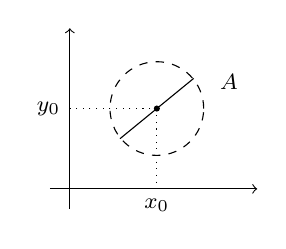
\begin{tikzpicture}[scale=0.85]
    \draw[->] (-0.3,0) -- (2.8,0);
    \draw[->] (0,-0.3) -- (0,2.4);
    \draw[dashed] (1.3,1.2) circle (0.7);
    \fill (1.3,1.2) circle (1.3pt);
    \draw (0.75,0.75) -- (1.85,1.65);
    \draw[dotted] (1.3,1.2) -- (1.3,0) node[below] {\footnotesize $x_0$};
    \draw[dotted] (1.3,1.2) -- (0,1.2) node[left] {\footnotesize $y_0$};
    \node[right] at (2.1,1.6) {\footnotesize $A$};
\end{tikzpicture}
\end{center}

Considero $F(t) = f(x_0 + th, y_0 + tk)$, $t \in [-1, 1]$ \pencilnote{($\sqrt{h^2 + k^2} < \delta$, così sto sempre nell'intorno)}.

$F(t) \in C^2([-1, 1])$ e ha un minimo in $t = 0$ \pencilnote{($(x_0, y_0)$)}.

Dunque
\[
F'(0) = 0 \quad (\implies \nabla f(x_0, y_0) = 0) \qquad \text{e} \qquad F''(0) \ge 0
\]
Dalla formula di Taylor:
\[
f(x_0 + h, y_0 + k) - f(x_0, y_0) = \langle \nabla f(x_0, y_0), (h, k) \rangle + \frac{1}{2} \underbrace{\left[ f_{xx}(x_0, y_0)\, h^2 + 2 f_{xy}(x_0, y_0)\, hk + f_{yy}(x_0, y_0)\, k^2 \right]}_{F''(0)} + o(h^2 + k^2) \ge 0
\]
\[
F''(0) = f_{xx}(x_0, y_0)\, h^2 + 2 f_{xy}(x_0, y_0)\, hk + f_{yy}(x_0, y_0)\, k^2 \ge 0 \qquad \forall h, k
\]
\pencilnote{Nota bene: non c'è l'$o(h^2 + k^2)$, poiché vale $\forall h, k$.}
\begin{itemize}
    \item Se $k = 0$ ho: $f_{xx}(x_0, y_0)\, h^2 \ge 0 \implies f_{xx}(x_0, y_0) \ge 0$
    \item Se $k \neq 0 \implies f_{xx}(x_0, y_0)\, \dfrac{h^2}{k^2} + 2 f_{xy}(x_0, y_0)\, \dfrac{h}{k} + f_{yy}(x_0, y_0) \ge 0$
\end{itemize}
Sia $\dfrac{h}{k} = t$:
\[
\implies a t^2 + 2b t + c \ge 0 \quad \forall t \implies \frac{\Delta}{4} \le 0 \implies b^2 - ac \le 0 \implies
\]
\[
\implies f_{xy}^2(x_0, y_0) - f_{xx}(x_0, y_0) f_{yy}(x_0, y_0) \le 0 \implies -H_f(x_0, y_0) \le 0 \implies H_f(x_0, y_0) \ge 0
\]
\end{proof}

\begin{example}
$f(x, y) = x^3 + y^3$, \quad $\nabla f = (3x^2, 3y^2)$

$(x_0, y_0) = (0, 0) \implies 1)\ \nabla f(0, 0) = (0, 0)$
\[
D^2 f = \begin{pmatrix} 6x & 0 \\ 0 & 6y \end{pmatrix}\Bigg|_{(0, 0)} = \begin{pmatrix} 0 & 0 \\ 0 & 0 \end{pmatrix} \implies H_f = 0, \quad f_{xx} \ge 0
\]
\end{example}

\begin{oss}
$H_f \ge 0 \implies f_{xx} f_{yy} - f_{xy} f_{yx} \ge 0 \implies f_{xx} f_{yy} - f_{xy}^2 \ge 0 \implies f_{xx} f_{yy} \ge f_{xy}^2 \ge 0 \implies f_{xx}, f_{yy}$ devono essere concordi, dunque mi basta chiedere il segno di una sola delle due (scelgo $f_{xx}$).
\end{oss}

\begin{theorem}[Cond. suff. al II° ordine ($n = 2$)]
Se $f : A \subseteq \mathbb{R}^2 \to \mathbb{R}$, $A \neq \emptyset$, $A$ aperto, $f \in C^2(A)$:

Se $(x_0, y_0) \in A$:
\begin{itemize}
    \item $\begin{cases} \nabla f(x_0, y_0) = (0, 0) \\ H_f(x_0, y_0) > 0 \\ f_{xx}(x_0, y_0) > 0 \end{cases} \implies (x_0, y_0)$ pto di min rel
    \item $\begin{cases} \nabla f(x_0, y_0) = (0, 0) \\ H_f(x_0, y_0) > 0 \\ f_{xx}(x_0, y_0) < 0 \end{cases} \implies (x_0, y_0)$ pto di max rel
    \item $\begin{cases} \nabla f(x_0, y_0) = (0, 0) \\ H_f(x_0, y_0) < 0 \end{cases} \implies (x_0, y_0)$ non è né min né max.
\end{itemize}
$\implies$ se $H_f(x_0, y_0)$ è nullo il teo non si applica $\implies$ bisogna usare la def. di estremo relativo!!!
\end{theorem}

\begin{example}
$f(x, y) = x^2 - y^2 \implies D^2 f = \begin{pmatrix} 2 & 0 \\ 0 & -2 \end{pmatrix}$, \quad $H_f(0, 0) = -4 < 0 \implies (0, 0)$ non è né max né min.
\end{example}

\begin{esercizio}
$f(x, y) = x y^2 e^{x - y}$, \qquad $A = \mathbb{R}^2$

Class. i pti critici:
\[
\begin{cases}
f_x = 0 \\
f_y = 0
\end{cases}
\iff
\begin{cases}
y^2 e^{x - y} + x y^2 e^{x - y} = 0 \\
2xy e^{x - y} - x y^2 e^{x - y} = 0
\end{cases}
\iff
\begin{cases}
y^2 (1 + x) = 0 \\
xy (2 - y) = 0
\end{cases}
\implies
\]
\[
\implies
\begin{cases}
y = 0 \\
\forall x \in \mathbb{R}
\end{cases}
\lor
\begin{cases}
1 + x = 0 \\
2xy (2 - y) = 0
\end{cases}
\xrightarrow{\text{supp. } y \neq 0 \text{ poiché } y = 0 \text{ già coperto a sx}}
\begin{cases}
1 + x = 0 \\
2 - y = 0
\end{cases}
\]
\[
P_x = (x, 0) \quad ; \quad Q(-1, 2)
\]
Es. per classificare $Q$ e $P_x$:
\begin{itemize}
    \item per $Q$ \pencilnote{(uso 2° teo)}: $H_f(Q) > 0, \ f_{xx}(Q) > 0 \implies Q$ è min rel
    \item per $P_x$: $\implies$ è difficile (vediamo la prox lez)
\end{itemize}
\end{esercizio}

\begin{solution*}[Risoluzione esercizio (23/10)]
Riprendiamo $f(x, y) = x y^2 e^{x - y}$:
\begin{align*}
f_x &= y^2 e^{x - y} + x y^2 e^{x - y} \\
f_y &= 2xy e^{x - y} - x y^2 e^{x - y}
\end{align*}
Calcoliamo le derivate seconde:
\begin{align*}
f_{xx} &= 2y^2 e^{x - y} + x y^2 e^{x - y} \\
f_{xy} = f_{yx} &= 2y e^{x - y} - y^2 e^{x - y} + 2xy e^{x - y} - x y^2 e^{x - y} \\
f_{yy} &= 2x e^{x - y} - 2xy e^{x - y} - 2xy e^{x - y} + x y^2 e^{x - y}
\end{align*}
Valutate in $P_x(x, 0)$:
\[
f_{xx}(x, 0) = 0, \qquad f_{xy}(x, 0) = 0, \qquad f_{yy}(x, 0) = 2x e^x
\]
\[
\implies D^2 f(x, 0) = \begin{pmatrix} 0 & 0 \\ 0 & 2x e^x \end{pmatrix}, \qquad H_f(x, 0) = 0
\]
Valutate in $Q = (-1, 2)$:
\begin{align*}
f_{xx}(Q) &= 4 e^{-3} \\
f_{yx}(Q) = f_{xy}(Q) &= e^{-3}(0) = 0 \\
f_{yy}(Q) &= e^{-3}(2) = 2 e^{-3}
\end{align*}
\[
D^2 f(Q) = \begin{pmatrix} 4 e^{-3} & 0 \\ 0 & 2 e^{-3} \end{pmatrix} \implies H_f(Q) > 0, \quad f_{xx} > 0 \implies \text{min rel}
\]
Per $P_x = (x, 0)$ usiamo la def.:
\[
\Delta f = f(x, y) - \underbrace{f(P_x)}_{= 0} = x y^2 e^{x - y} \ge 0 \iff x \ge 0
\]
\begin{center}
\begin{tikzpicture}[scale=0.85]
    \draw[->] (-1.8,0) -- (1.8,0) node[right] {$x$};
    \draw[->] (0,-1.4) -- (0,1.4) node[above] {$y$};
    \foreach \x in {-1.2,-0.8,-0.4,0,0.4,0.8,1.2} {
        \draw (\x,0) circle (1.5pt);
    }
    \node at (0.85,0.65) {\footnotesize $+$};
    \node at (0.85,-0.65) {\footnotesize $+$};
    \node at (-0.85,0.65) {\footnotesize $-$};
    \node at (-0.85,-0.65) {\footnotesize $-$};
\end{tikzpicture}
\end{center}
\[
P_x = (x, 0) : \begin{cases}
x > 0 & \text{pti di min relativo} \\
x < 0 & \text{pti di max relativo} \\
x = 0 & \text{né min né max}
\end{cases}
\]
\end{solution*}



\begin{definition}[Matrice def. pos.]
$A = \{ a_{ij} \}$, $A$ quadrata di ordine $m$:
\begin{itemize}
    \item simm. e tutti gli autovalori positivi $\implies$ si dice \underline{definita positiva}
    \item simm. e tutti gli autovalori negativi $\implies$ si dice \underline{definita negativa}
\end{itemize}
Supp. $m = 2 \implies A > 0 \iff \det A > 0$ e $a_{11} > 0$.

$m = 3 \implies A > 0 \iff$
\[
\det A > 0, \qquad \det A_{11} = a_{11} > 0, \qquad \det A_{22} = a_{11} a_{22} - a_{12}^2 > 0
\]
\[
\begin{pmatrix}
\boxed{a_{11}} & a_{12} & a_{13} \\
a_{12} & a_{22} & a_{23} \\
a_{13} & a_{23} & a_{33}
\end{pmatrix}
\]
Per la definita negatività:
\begin{itemize}
    \item $m = 2$: $A < 0 \iff \begin{cases} \det A > 0 \\ a_{11} < 0 \end{cases}$
        \item $m = 3$: $A < 0 \iff \begin{cases} \det A < 0 \\ a_{11} < 0 \\ \det A_{22} > 0 \implies a_{11} a_{22} - a_{12}^2 > 0 \end{cases}$
\end{itemize}
\pencilnote{Nota: per il lemma $\displaystyle\sum_{i,j=1}^m a_{ij} v_i v_j > 0$ $\ \forall v \neq 0$ (forma quadratica).}
\end{definition}

\subsection{Esercizi}

\begin{esercizio}
Classificare i punti critici (e gli assoluti per il 3):
\begin{enumerate}
    \item $f(x, y) = 4x^2 - 4x^2 y^2 - x^4$
    \item $f(x, y) = y^3 + (x - y)^2$
    \item $f(x, y) = 2xy - x^2 - y^4$ \quad e poi gli assoluti in $Q = [0, 1]^2$.
\end{enumerate}

\textbf{1)}
\[
\begin{cases}
f_x = 8x - 8x y^2 - 4x^3 = 0 \\
f_y = -8x^2 y = 0 \to x = 0 \text{ oppure } y = 0
\end{cases}
\implies
\begin{cases}
x = 0 \\
\forall y
\end{cases}
\cup
\begin{cases}
y = 0 \\
2 - x^2 = 0
\end{cases}
\begin{aligned}
&\to Q_1 = (\sqrt{2}, 0) \\
&\to Q_2 = (-\sqrt{2}, 0)
\end{aligned}
\]
Dal primo sistema: retta $P_y(0, y)$ $\forall y \in \mathbb{R}$.
\begin{align*}
f_{xx} &= 8 - 8y^2 - 12x^2 \\
f_{xy} = f_{yx} &= -16xy \\
f_{yy} &= -8x^2
\end{align*}
Valutate in $(0, y)$: $f_{xx}(0, y) = 8 - 8y^2$, $f_{xy}(0, y) = 0$, $f_{yy}(0, y) = 0 \implies H_f(P_y) = 0$.

Valuto in $Q_1$:
\[
f_{xx}(Q_1) = -16, \quad f_{yx} = f_{xy} = 0, \quad f_{yy} = -16 \implies H_f(Q_1) = 16^2 > 0, \quad f_{xx} = -16 < 0 \implies \text{è max rel.}
\]
$H_f(Q_2) > 0, \ f_{xx} < 0 \implies$ è max rel.

Per la retta uso la def.: $\Delta f = f(x, y) - \underbrace{f(P_y)}_{= 0} \ge 0 \implies$
\[
\Delta f = 4x^2 - 4x^2 y^2 - x^4 \ge 0 \implies 4 - 4y^2 - x^2 \ge 0 \implies \frac{x^2}{4} + \frac{y^2}{1} \le 1
\]
\begin{center}
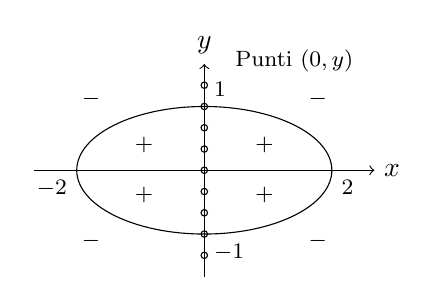
\begin{tikzpicture}[scale=0.9]
    \draw[->] (-2.4,0) -- (2.4,0) node[right] {$x$};
    \draw[->] (0,-1.5) -- (0,1.5) node[above] {$y$};
    \draw (0,0) ellipse (1.8 and 0.9);
    \foreach \y in {-1.2,-0.9,-0.6,-0.3,0,0.3,0.6,0.9,1.2} {
        \draw (0,\y) circle (1.3pt);
    }
    \node[below right] at (1.8,0) {\footnotesize $2$};
    \node[below left] at (-1.8,0) {\footnotesize $-2$};
    \node[above right] at (0,0.9) {\footnotesize $1$};
    \node[below right] at (0,-0.9) {\footnotesize $-1$};
    \node[above right] at (0.3,1.25) {\footnotesize \pencilnote{Punti $(0, y)$}};
    \node at (0.85,0.35) {\footnotesize $+$};
    \node at (-0.85,0.35) {\footnotesize $+$};
    \node at (0.85,-0.35) {\footnotesize $+$};
    \node at (-0.85,-0.35) {\footnotesize $+$};
    \node at (1.6,1.0) {\footnotesize $-$};
    \node at (-1.6,1.0) {\footnotesize $-$};
    \node at (1.6,-1.0) {\footnotesize $-$};
    \node at (-1.6,-1.0) {\footnotesize $-$};
\end{tikzpicture}
\end{center}
\[
\implies P_y(0, y) = \begin{cases}
-1 < y < 1 & \to \text{min rel} \\
y < -1 \lor y > 1 & \to \text{max rel}
\end{cases}
\qquad \text{e } (0, \pm 1) \text{ non è né max né min.}
\]

\textbf{2)} $f(x, y) = y^3 + (x - y)^2$
\[
\begin{cases}
f_x = 2(x - y) = 0 \\
f_y = 3y^2 - 2(x - y) = 0
\end{cases}
\to
\begin{cases}
y = 0 \\
2(x - y) = 0
\end{cases}
\to (0, 0)
\]
\[
f_{xx} = 2, \qquad f_{xy} = f_{yx} = -2, \qquad f_{yy} = 6y + 2
\]
Valuto in $(0, 0)$: $f_{xx}(0, 0) = 2$, $f_{xy} = f_{yx}(0, 0) = -2$, $f_{yy} = 2 \implies H_f(0, 0) = 4 - 4 = 0$.
\[
\Delta f = f(x, y) - f(0, 0) = f(x, y) \ge 0 \iff y^3 + (x - y)^2 \ge 0
\]
Mi metto sulla bisettrice $\implies (x - y)^2 = 0 \implies y^3 \ge 0 \implies$ in $O$ non ho né un min né un max \pencilnote{(rivedi bene)}.
\end{esercizio}
